\documentclass[11pt]{article}
\usepackage[a4paper,left=1in,right=1in,top=1in,bottom=1in]{geometry}

\usepackage[english]{babel}
\usepackage[T1]{fontenc}
\usepackage[utf8]{inputenc}
\usepackage{seqsplit}

\renewcommand{\familydefault}{\sfdefault}
\usepackage{setspace}  \singlespacing
\usepackage{graphicx}
\usepackage[absolute]{textpos}
\usepackage{xcolor}
\usepackage{fontawesome5}
\usepackage{multirow}
\usepackage{hyperref}
\usepackage{tcolorbox}
\hypersetup{
    colorlinks,
    linkcolor={red!50!black},
    citecolor={blue!50!black},
    urlcolor={blue}
}

\definecolor{mgray}{gray}{0.85}
\definecolor{mpurple}{HTML}{68236D}
\usepackage{float}
\usepackage{subfig,wrapfig}
\usepackage{amsmath,amsfonts,amsthm,amssymb}
\usepackage{fancyhdr,fancybox,color}
\usepackage{enumerate}
\usepackage[amssymb]{SIunits}
\definecolor{MyBlue}{rgb}{0,0.3,0.6}
\usepackage[all]{hypcap}
\usepackage{csquotes}
\usepackage[url=false,
backend=bibtex,
style=authoryear-comp,
doi=true,
isbn=true,
backref=false,
dashed=false,
maxcitenames=2,
maxbibnames=99,
natbib=true]{biblatex}
\DeclareNameAlias{author}{family-given}
\renewbibmacro{in:}{}
\addbibresource{../_logosAndRef/references.bib}
\nonfrenchspacing

\newlength{\headertobodysep}
\setlength{\headertobodysep}{1cm}

\begin{document}
\thispagestyle{empty}

\textblockorigin{0pt}{0pt}

\begin{textblock*}{5cm}(0.5cm,1cm)
    
\includegraphics[height=2cm]{../_logosAndRef/Durham-University.pdf}
\end{textblock*}

\begin{textblock*}{9cm}(6cm,1.5cm)
    \centering
    {\large \textbf{Wafer Bonding | CoMPhy Lab}}\\[0.2em]
    Department of Physics, Durham University\\[0.3em]
    \href{https://comphy-lab.org}{comphy-lab.org}
\end{textblock*}

\begin{textblock*}{5cm}(15.5cm,1cm)
    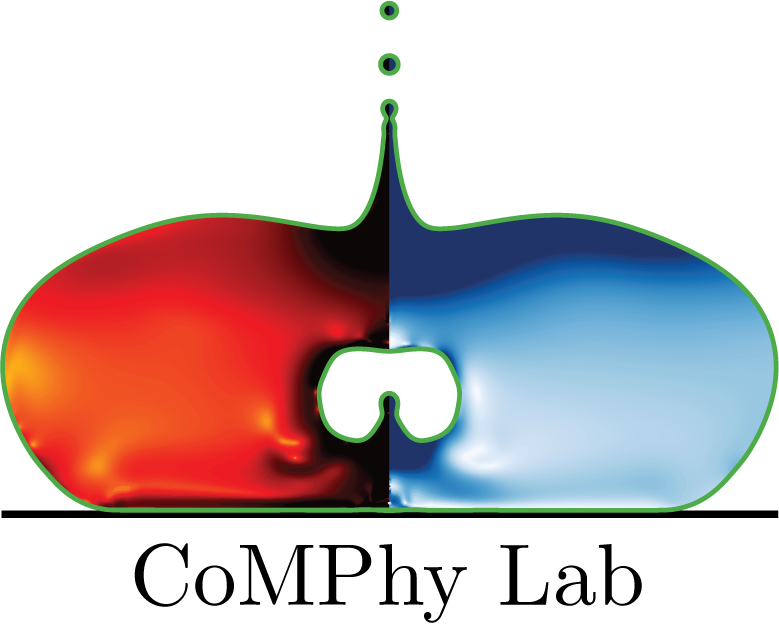
\includegraphics[height=2cm]{../_logosAndRef/CoMPhy-Lab.png}
\end{textblock*}

\vspace*{\headertobodysep}

\begin{center}
    \begin{LARGE}
     A table-top probe of wafer bonding: AFM and nanoscale gas drainage
    \end{LARGE}
\end{center}

\noindent Hybrid-bonded chips rely on two ultraflat silicon wafers snapping together while trapped gas escapes through a closing nanometre gap. Get the local drainage physics wrong, and the bond front leaves a void that kills the die. A wafer-scale bond event couples long-range elastic plate bending and an autonomous front-speed selection to a local drainage law in the closing nanometre gap; that local law is the closure every continuum bond-front model inherits~\citep{rieutord2005bondwave,navarro2013coupledbonding}. This project isolates it. The single-asperity geometry is the minimal model: stripping the wafer-scale elasticity and autonomous front propagation out leaves the nanoscale squeezed-film law in the $\mathrm{Kn} \sim \mathcal{O}(1)$ regime, in its cleanest form. A heavily blunted atomic force microscope (AFM) tip, pressed against a polished substrate under controlled humidity, delivers a clean single-asperity realisation of that drainage law; axisymmetric direct numerical simulations of the same geometry close the loop.

\begin{tcolorbox}[colback=mgray,colframe=mpurple,title=TL;DR]
You will run AFM force-distance experiments (with Dr~Kislon~Vo\"itchovsky, Durham) using a heavily blunted tip pressed against a flat substrate under a humidity sweep from dry nitrogen ($<5\%$ RH) upward, and you will build direct numerical simulations (with Dr~Vatsal~Sanjay, CoMPhy Lab) of the squeezed film between tip and substrate. The two sides meet at a quantitative test of the nanoscale drainage constitutive law in the $\mathrm{Kn} \sim 1$ slip regime --- the same sub-continuum piece that controls void formation and bond-wave distortion in industrial hybrid bonding at imec and TSMC~\citep{nagano2022voidformation,sato2025bondwave}. This is the minimal model: the local drainage law, isolated from wafer-scale bending elasticity, that a Rieutord--Navarro bond-front solver needs as closure input.
\end{tcolorbox}

\section*{Description}

Direct wafer bonding is the process by which two polished semiconductor wafers are brought into contact and seal together through van der Waals and capillary forces, with the ambient gas expelled radially as a bond wave propagates from an initial contact point~\citep{plosslKrauter1999,masteika2014waferbonding,gosele1995bondingspeed}. The established front-speed scaling, derived by Rieutord and collaborators for flexible silicon wafers separated by a thin fluid layer, is $v \propto w^{5/4}$ with $w$ the wafer thickness~\citep{rieutord2005bondwave}; the most complete published model couples plate-bending theory to Reynolds lubrication and an adhesion-front boundary condition~\citep{navarro2013coupledbonding}. The industrial figures of merit are not overlay alone (overlay is a downstream alignment metric) but \emph{void density, unbonded area}, and \emph{bond-wave-induced distortion}~\citep{nagano2022voidformation,sato2025bondwave}. Each of these is controlled by what happens inside the closing gap. As the gap approaches the molecular mean free path ($\lambda \approx 68$\,nm for air at STP), Knudsen slip, rarefaction, and sub-continuum gas dynamics all enter, and a naive continuum Reynolds closure drifts. Real closing gaps live at Knudsen numbers $\mathrm{Kn} = \lambda/h \sim \mathcal{O}(1)$: a regime that is neither continuum nor free-molecular, and where the appropriate closure is the Fukui--Kaneko generalised lubrication equation tabulated from DSMC-validated Poiseuille coefficients~\citep{fukuiKaneko1988, fukuiKaneko1990}.

The bond-wave physics is hard to probe on a production scanner --- the gap is buried between two 300\,mm wafers and closes in milliseconds. An AFM single-asperity geometry is the minimal model by construction: stripping out wafer-scale bending and autonomous front propagation isolates the same nanoscale squeezed-film law that a continuum bond-front model takes as its closure. A standard AFM cantilever has a tip radius of $\mathcal{O}(10)$\,nm; deliberately blunting it~\citep{butt2005forcemicroscopy} to $\mathcal{O}(1\text{--}10)$\,\micro m produces a hemispherical punch of known radius~$R$, which can be driven against a polished substrate at controlled approach velocity $U$ under controlled humidity~\citep{buttKapplSurfaceForces2018}. The force-distance curve carries three separable signatures: (i) pre-contact capillary jump-in at humidity-set separations~\citep{israelachvili2011}, (ii) squeezed-film viscous resistance that follows Stefan's law $F_{\mathrm{visc}} = 3\pi \eta R^2 U / (2h)$ (sphere-on-flat, thin-gap) at low $\mathrm{Kn}$ but drifts predictably as slip enters at $h \lesssim \lambda$, and (iii) a pull-off force set by JKR or DMT adhesion~\citep{maugis1992adhesion}, modulated by any condensed bridge formed during contact. The AFM sweep maps the local constitutive law $F(h; \mathrm{Kn}, \mathrm{Ca}, \mathrm{RH})$ --- where $\mathrm{Ca} = \eta U / \gamma$ --- not the front itself. The mapping to industrial bonding is indirect but concrete: once the local drainage law is quantified, it can be embedded as the closure in a bond-front solver of the Rieutord--Navarro class.

%-------------------------------------------------------------------
% FIGURE 1 -- Multi-scale bridge from wafer bond front to AFM experiment
% Suggested two-panel comparison, same physics, different scale:
%   (a) Wafer bond front: two 300mm wafers with an initial contact point
%       near the centre, bond front propagating radially, trapped gas
%       ahead of the front. Mark U, gap h, mean free path lambda, and
%       wafer flexural length L_w = (E t^3 / gamma_s)^{1/4}.
%   (b) AFM experiment: blunted tip (radius R ~ 1-10 um), flat
%       substrate, capillary bridge at tip/substrate junction, labelled
%       R, h, theta_e, humidity RH.
% Caption: the same three-force balance (adhesion, capillarity,
% viscous/rarefied-gas drainage) governs both systems; the AFM gives
% controlled, repeatable access to it.
%-------------------------------------------------------------------
\begin{figure}[H]
    \begin{center}
        % \includegraphics[width=\textwidth]{bond_front_vs_AFM.pdf}
        \fbox{\parbox[b][4cm][c]{0.95\textwidth}{\centering\small\emph{Placeholder for two-panel schematic: (a) wafer bond-wave geometry (bending plates + lubricating gas layer + advancing adhesion front), (b) blunted-AFM single-asperity geometry isolating the nanoscale squeezed-film law that feeds (a).}}}
        \caption{The AFM is a local constitutive probe, not a full bond-wave analogue. Panel (a) shows the wafer-scale problem: two bending plates, a lubricating gas layer, an autonomously propagating adhesion front. Panel (b) shows the single-asperity AFM geometry that isolates the thin-gap drainage law $F(h; \mathrm{Kn}, \mathrm{Ca}, \mathrm{RH})$ entering (a) as a closure.}
        \label{fig:bridge}
    \end{center}
\end{figure}

This project closes that local loop. On the experimental side, you will run force-distance curves with a blunted AFM tip on silicon and oxide-terminated substrates, sweeping both approach speed (four decades, $10^{-9}$ to $10^{-5}$\,m\,s$^{-1}$) and relative humidity (from $<5\%$ dry-nitrogen purge upward in steps, so gas drainage and capillary condensation are separable in the data, not conflated~\citep{butt2005forcemicroscopy}). On the theoretical side, you will build axisymmetric direct numerical simulations in Basilisk C~\citep{popinet2015quadtree,basiliskVatsal} of the closing gap, with the Fukui--Kaneko slip-corrected lubrication closure for the gas phase to cover the continuum-to-rarefied transition~\citep{fukuiKaneko1988, fukuiKaneko1990}, and a disjoining-pressure potential $\Pi(h)$ with $\int \Pi\,dh = W_{\mathrm{adh}}$ as the molecular-adhesion closure. The experiment and the simulation meet at one non-trivial prediction: the speed and humidity dependence of the squeezed-film force at $\mathrm{Kn} \sim 1$. The tested closure then feeds back into bond-wave models of the Rieutord--Navarro class.

%-------------------------------------------------------------------
% FIGURE 2 -- AFM force-distance schematic (to draw)
% Panels:
%   (a) Idealised force-distance trace: approach (gray dashed), jump-in,
%       contact region, retraction (solid), pull-off peak. Mark the
%       three signatures (capillary jump-in, viscous drainage, pull-off).
%   (b) Cartoon of blunted tip near substrate showing gap, capillary
%       meniscus at high RH, and far-field gas flow.
%-------------------------------------------------------------------
\begin{figure}[H]
    \begin{center}
        % \includegraphics[width=0.9\textwidth]{afm_fd_curves.pdf}
        \fbox{\parbox[b][4cm][c]{0.9\textwidth}{\centering\small\emph{Placeholder: (a) idealised approach/retraction force-distance trace with annotated regimes, (b) blunted-tip-on-substrate schematic with meniscus, squeezed gap, and Knudsen-slip region.}}}
        \caption{AFM force-distance signature of the three-force balance. Capillary jump-in (high RH, low $U$), viscous drainage (high $U$, continuum), and pull-off (adhesion-dominated retraction) are separable regimes of the same underlying model.}
        \label{fig:afm-fd}
    \end{center}
\end{figure}

%-------------------------------------------------------------------
% FIGURE 3 -- Regime map in (Ca, Kn) space with industrial targets
% Axes: log Ca, log Kn. Regions: continuum viscous (low Kn, any Ca),
% Knudsen slip (Kn ~ O(1)), free-molecular (high Kn). Mark:
%   - 300mm wafer bond front at industrial speed (reference point)
%   - Target imec overlay regime
%   - Accessible AFM sweep region
% Shows that AFM sweep overlaps the industrially relevant region.
%-------------------------------------------------------------------
\begin{figure}[H]
    \begin{center}
        % \includegraphics[width=0.7\textwidth]{ca_kn_map.pdf}
        \fbox{\parbox[b][4cm][c]{0.7\textwidth}{\centering\small\emph{Placeholder: $(\mathrm{Ca}, \mathrm{Kn})$ regime map showing wafer bond front, industrial hybrid-bonding target, and the portion accessible with blunted AFM.}}}
        \caption{Dimensionless map. The blunted-AFM sweep covers the industrially relevant $\mathrm{Ca}$-$\mathrm{Kn}$ corner where continuum lubrication theory fails and sub-continuum gas physics sets the bond-front velocity. This is the target of the project.}
        \label{fig:regime-map}
    \end{center}
\end{figure}

\section*{What you will do and what you will learn?}

\begin{enumerate}
\itemsep0em
\item Learn force-spectroscopy AFM in Dr~Vo\"itchovsky's lab: cantilever calibration, tip blunting protocols, humidity-controlled force-distance measurements, and data reduction from raw deflection to force.
\item Build an axisymmetric Basilisk C simulation of a blunted-tip approach to a flat substrate, with a slip-corrected Reynolds layer for the gas phase and a meniscus model for condensed water. Follow the CoMPhy-Lab two-phase and documentation conventions~\citep{basiliskVatsal,basiliskVatsalDropFilm}.
\item Derive the local squeezed-film law in the three canonical limits --- continuum Stefan ($\mathrm{Kn} \to 0$), Knudsen slip ($\mathrm{Kn} \sim 1$), and capillary-bridge dominated (high RH, low $U$). Test the Fukui--Kaneko generalised lubrication closure~\citep{fukuiKaneko1988,fukuiKaneko1990} against the force-distance data, identify where it drifts, and bracket its quantitative validity range in $\mathrm{Kn}$. Place the measured $F(h; \mathrm{Kn}, \mathrm{Ca}, \mathrm{RH})$ alongside the established wafer-scale front-speed scaling $v \propto w^{5/4}$~\citep{rieutord2005bondwave}, treating the AFM data as a direct measurement of the local drainage closure that Rieutord--Navarro-class bond-wave solvers require as input.
\item Position the results in the wafer-bonding landscape through the primary literature: the Rieutord 5/4 derivation~\citep{rieutord2005bondwave}, the Navarro coupled plate-bending / lubrication model~\citep{navarro2013coupledbonding}, the G\"osele--Tong bond-speed analysis~\citep{gosele1995bondingspeed}, Masteika's review~\citep{masteika2014waferbonding}, and the Nagano and Sato process-yield studies that actually quantify the industrial figures of merit~\citep{nagano2022voidformation,sato2025bondwave}. Write a short section of the final report on how the measured local drainage closure feeds a bond-front solver and which sub-100-nm physics it fixes for the wafer-scale problem.
\item Develop the CoMPhy-Lab full-stack open-source skillset: Basilisk, adaptive mesh refinement, Python post-processing, GitHub documentation, and writing for a combined soft-matter and semiconductor-physics audience.
\end{enumerate}

\section*{Industrial and scientific context}

Hybrid bonding is the enabling technology for 3D-stacked logic, high-bandwidth memory, and backside power delivery in the sub-2\,nm node. TSMC's SoIC and Intel's Foveros both use it in volume. The dominant yield-limiting failure modes reported in the public process-engineering literature are not overlay error but \emph{void formation}, \emph{unbonded area}, and \emph{bond-wave-induced in-plane distortion}~\citep{nagano2022voidformation,sato2025bondwave}; overlay is the downstream alignment metric that these upstream failures corrupt. Each of these failures is seeded inside the closing gap, where sub-continuum gas drainage at Knudsen numbers around unity sets whether the front sweeps cleanly or pockets gas. Existing continuum-Reynolds closures in bond-front solvers of the Rieutord--Navarro class~\citep{rieutord2005bondwave,navarro2013coupledbonding} do not cover that regime; the Fukui--Kaneko generalised lubrication equation does, but it has not been directly benchmarked against a controlled single-asperity experiment in the relevant $\mathrm{Kn}$ range. The blunted-AFM setup is a clean-boundary-condition minimal model: it isolates the local closure and feeds it back to the wafer-scale solver. For a Durham MPhys or Master's project, this gives a crisp deliverable: a quantified drainage law at $\mathrm{Kn} \sim 1$, paired simulation and experiment, and an honest mapping onto a named industrial yield metric.

If you have any questions, feel free to contact us \href{mailto:vatsal.sanjay@comphy-lab.org}{vatsal.sanjay@comphy-lab.org}/\\\href{mailto:vatsal.sanjay@durham.ac.uk}{vatsal.sanjay@durham.ac.uk} or drop by Ph255 (Rochester building) at the Department of Physics at Durham University.

\begin{center}
\begin{tabular}{|l|l|l|}
\hline \textbf{Collaborators} & \textbf{E-mail} & \textbf{Based at} \\
\hline \multirow{2}{*}{Dr. Vatsal Sanjay} & \href{mailto:vatsal.sanjay@comphy-lab.org}{vatsal.sanjay@comphy-lab.org} & \multirow{2}{*}{Ph255 (Rochester building)} \\
& \href{mailto:vatsal.sanjay@durham.ac.uk}{vatsal.sanjay@durham.ac.uk} & \\
\hline Dr. Kislon Vo\"itchovsky & \href{mailto:kislon.voitchovsky@durham.ac.uk}{kislon.voitchovsky@durham.ac.uk} & Dept. of Physics, Durham \\
\hline Dr. Utkarsh Jain & \href{mailto:utkarsh.jain@imec.be}{utkarsh.jain@imec.be} & imec, Leuven \\
\hline
\end{tabular}
\end{center}

\vspace{1em}
\noindent\textit{Last updated: \today}

\printbibliography

\end{document}
